\subsection{Online Execution}
\label{sec_online_execution}

Following the idea of solving the problem in the dual domain, this section presents an algorithm that approximates gradient descent on the dual domain in the online stage. To be formal define the dual function as $d(\lambda) := \max_{\pi} \mathcal{L}(\pi,\lambda),$ with $\mathcal{L}(\pi,\lambda)$ as in \eqref{eqn_lagrangian}.
According to Danskin's Theorem \cite{danskin1966theory} the minimization of the dual  over $ \lambda\geq 0$, can be achieved by substituting the constraints evaluated at the optimal policy for the gradient of $d(\lambda)$ to obtain the dual gradient update $\lambda_{k+1} = \left[\lambda_{k}-\eta\left(V\left(\pi\left[\lambda_{k},\ldots,\lambda_k\right]\right)-c\right)\right]_+,$ where $[\cdot]_+$ denotes the projection on the non-negative orthant.

For a data-driven implementation, we run stochastic gradient descent  \cite{dvoretsky1955stochastic}, dropping the expectation and replacing it with reward samples. As we did for training, we also set a finite horizon $T_0$.    Hence, we use the following stochastic dual update 
\begin{align}\label{eqn_contractive_big_brother}
    \lambda_{k+1} = \left[(1-\alpha) \lambda_k + \frac{\eta}{T_0} \sum_{\tau=k T_0}^{(k+1) T_0-1}\left(c-r(S_\tau) \right)\right]_{+},
\end{align}
introducing also a contractive factor $(1-\alpha)$, with $\alpha\in(0,1)$, which will be necessary to ensure that the errors induced by the stochastic communication graph do not grow unbounded, as we discuss on the remark at the end of this section.

The stochastic update in \eqref{eqn_contractive_big_brother} can be incorporated into the MDP modeling $S_t$ to form an augmented dynamical system with state  $(S_t,\lambda_k)$ in two timescales, with $t$ representing the time step and $k$ indexing the rollout, which spans $T_0$ time steps from $kT_0$ to $(k+1)T_0-1$. 

During the execution phase, the agents cannot observe global rewards, which are available locally only to the agents whose states $S_t^n$ are in regions $\mathcal S_m$. Hence, the update in \eqref{eqn_contractive_big_brother} is not realizable. Instead, agents exchange the reward information across the communication network to implement \eqref{eqn_contractive_big_brother} in a distributed manner. To devise such a distributed procedure, define $R_{\tau,t}^n\in\mathbb{R}^M$ as the estimate that the agent $n$ has at time $t$ about the actual value of the rewards $r(S_\tau)$ at a previous time $\tau\leq t$. The communication timeline is shown in Figure \ref{fig:timeline}.
%
\begin{figure}[t]
    \centering
    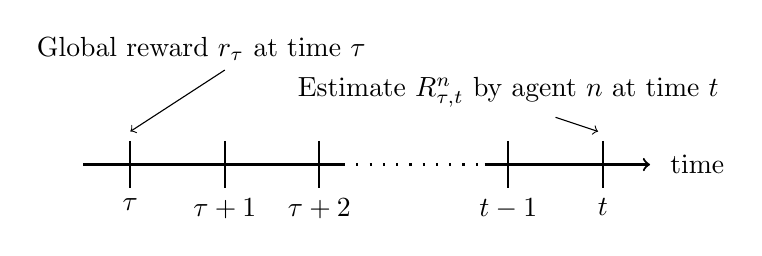
\begin{tikzpicture}[scale=0.6] % Smaller scale

    % Timeline with arrow
    \draw[black,thick, -] (-2.5,0) -- (3,0);
    \draw[black,thick, ->] (6,0) -- (9.5,0); % Horizontal line with arrow at the end

    % Markers with labels
    \draw[thick,black] (-1.5,0.5) -- (-1.5,-0.5) node[below] {$\tau$};
    \draw[thick,black] (0.5,0.5) -- (0.5,-0.5) node[below] {$\tau+1$};
    \draw[thick,black] (2.5,0.5) -- (2.5,-0.5) node[below] {$\tau+2$};

    % Dotted line for the break between $\tau+2$ and $T-1$
    \draw[loosely dotted,thick,black] (3,0) -- (6,0); % Dotted line between tau+2 and T-1

    % More markers and labels
    \draw[thick,black] (6.5,0.5) -- (6.5,-0.5) node[below] {$t-1$};
    \draw[thick,black] (8.5,0.5) -- (8.5,-0.5) node[below] {$t$};


    \node[above] at (0,2) {Global reward $r_\tau$ at time $\tau $};
    \draw[->] (0.5,2) -- (-1.5,0.7) ;

    % Agent n above T
    \node[above] at (6.5,1) {Estimate $R^n_{\tau,t}$ by agent $n$ at time $t$};
    \draw[->] (7.5,1) -- (8.4,0.7) ;

    % Arrow pointing to the end, with label t
    \node at (10.5,0) {time}; % Label 'time' at the end
    %\draw[thick, ->] (9, 0) -- (9.5, 0); % Arrow pointing to the right to indicate end
    
\end{tikzpicture}

    \caption{\emph{Gossip} timeline: Each agent aims to estimate the global vector of rewards $r(S_{\tau})$. After $t-\tau$ time steps, the local estimation of $r(S_{\tau})$ obtained by agent $n$ is $R_{\tau,t}^n$.}
    \label{fig:timeline} 
\end{figure}
%
Consider an agent $n^\prime$ whose state $S_\tau^{n^\prime}$ is in region $\mathcal S_m$  at time $\tau$. That is $S_\tau^{n^\prime}\in \mathcal S_m$ as shown in Figure~\ref{fig:gossip_stochastic} for the case of our monitoring Example \ref{example}. Then agent $n^\prime$ knows first-hand that the reward for the region $S_m$ is being attended at this specific time $\tau$, and thus the global reward $(r(S_{\tau}))_m = 1$ is being attained. Hence, it sets its own local estimate of the reward to one,  i.e., $(R_{\tau,t}^{n^\prime})_m = (r(S_{\tau}))_m = 1 \ \textrm{for all}\ t\geq \tau$. Then, it passes this information to its neighbors, who will update their local estimates of the reward $(r(S_{\tau}))_m$ accordingly. Specifically, each agent will receive the local estimates of $r(S_{\tau})$ from its neighbors and set its local estimate to $1$ if any of its neighbors have a local estimate of $1$ for the same region. That is equivalent to using the maximum of the local estimates of its neighbors, including itself. In general, the update rule for the local copies of the rewards is given by
%
\begin{align}\label{eqn_gossip_r}
    	\left(R_{\tau,t}^n\right)_m&=\begin{cases}
    	\textcolor{black}{\max_{n^\prime\in\mathcal N_n\cup \{n\}} \left(R_{\tau,t-1}^{n^\prime}\right)_m},& t>\tau\\
    	\mathds 1\{S_{t}^n\in\mathcal S_m\},& t=\tau,
    	\end{cases}
\end{align}
%
where $\mathcal N_n$ is the (stochastic, time-varying) neighborhood of agent $n$ at time $t$, and $\mathds 1\{S_{t}^n\in\mathcal S_m\}$ is the direct observation that the state of agent $n$ is in $\mathcal S_m$ at time $t$. During each rollout $k$, agent $n$ keeps the series of estimates $R_{\tau,t}^{n},\ \tau=kT_0,\ldots,(k+1)T_0-1 $, updating them recursively via \eqref{eqn_gossip_r} at each time $t=\tau,\ldots,(k+1)T_0-1$.

Using these \emph{gossiped} reward estimates to update the multipliers, the distributed version of \eqref{eqn_contractive_big_brother} becomes
%
\begin{align}\label{eqn_stochastic_dual}
    \lambda_{k+1}^n = \left[(1-\alpha) \lambda_k^n + \frac{\eta}{T_0} \sum_{\tau=k T_0}^{(k+1) T_0-1}\left(c-R_{\tau,(k+1)T_0-1}^n \right)\right]_{+}
\end{align}
%
where agent $n$ waits as much as possible until the end of the rollout at time $t=(k+1)T_0-1$ to substitute $R_{\tau,(k+1)T_0-1)}$ for $r(S_{\tau})$ and thus have the best possible estimate.  

Equations \eqref{eqn_gossip_r} and \eqref{eqn_stochastic_dual}, together with the policy structure in \eqref{eqn_separate_policy},  are the main tools for the distributed implementation of the dual update, allowing agents to run the fully distributed policy in Algorithm \ref{algo:alg_main_algorithm}.

\begin{algorithm}[t]
\caption{Distributed multi-agent  policy execution}\label{algo:alg_main_algorithm}
\begin{algorithmic}[1]
\FOR{$k=0,1,\ldots$}
  \STATE Substitute $\lambda^{k}_n$ in \eqref{eqn_optimal_trained_policy}  pretrained with local gradients.
  \STATE Keep the local realizable policy $\pi_{\theta^n}[\lambda^{k}_n]$ as in \eqref{eqn_realizable_policy}.
  \FOR{$t=k T_0,\ldots,(k+1)T_0-1$}
  	\STATE Act $A^n_t\sim \pi_{\theta^n}[\lambda^{k}_n]$ and transition to $S_{t+1}^n$.\\
    \STATE Collect local rewards $(R_{t,t}^n)_m=\mathds{1}\{S_t^n\in\mathcal S_m\}$. \\
  	\STATE \emph{Network gossiping:} Update $ R_{\tau,t}^n$ as in \eqref{eqn_gossip_r}.
  \ENDFOR
   \STATE Update the multipliers according to \eqref{eqn_stochastic_dual}.
\ENDFOR
\end{algorithmic}
\end{algorithm}

In executing Algorithm \ref{algo:alg_main_algorithm}, agents use a \emph{realizable} policy $\pi_{\theta}[\lambda^1,\ldots,\lambda^N]$ in the sense that it is parametric, trained with finite rollouts as in \eqref{eqn_optimal_trained_policy}, and with local copies of the multipliers. Specifically, each agent $n$ substitutes its local copy of the vector of multipliers $\lambda^n$ for $\lambda$ in \eqref{eqn_separate_policy} to obtain  its local part of the realizable policy  $\pi_{\theta^n}(A_t^n\mid S_t^n,\lambda^n)$. Accordingly, the realizable global policy corresponds to  their product
%
\begin{align}\label{eqn_realizable_policy}
\pi_\theta[\lambda^1,\ldots,\lambda^N](A_t\mid S_t)&:=\prod_{n=1}^N\pi_{\theta^n}(A_t^n|S_t^n,\lambda^n).
\end{align}

By using the  distributed policies in \eqref{eqn_realizable_policy}, the team achieves the following realizable value
\begin{align}\label{eq:non-idealities-VR}
V_R&:=V_{T_0}\left(\pi_\theta[\lambda_k^1 \ldots \lambda^N]\right)
=\mathbb E_{\pi_\theta}\left[\frac{1}{T_0} \sum_{t=k T_0}^{(K+1) T_0-1} r(S_t)\ \right].
\end{align}

Because agents cannot guarantee to reach exact consensus on the multipliers $\lambda^n$ almost surely when communicating over the stochastic graph \eqref{eqn_graph_model}, their realizable policies $\pi_{\theta^n}(\lambda^n)$ will differ from the one $\pi_{\theta^n}(\lambda)$ trained for, which assumed global access to $\lambda$. To mitigate the effect of this mismatch, we need the following assumption. 

\begin{assumption}[Lipschitz continuity of value functions]\label{assumption:lipschitz}
The difference between the value functions $V_P$ and $V_R$ with global and distributed multipliers, as defined in \eqref{eq:non-idealities-VP} and \eqref{eq:non-idealities-VR}, respectively, is bounded by the scaled difference  their multipliers with scaling constant $L>0$, i.e., 
\begin{align}
\nonumber \|V_P-V_R\|&=\|V_{T_0}(\pi_\theta[\lambda, \ldots, \lambda]) - V_{T_0}(\pi_\theta[\lambda^1, \ldots, \lambda^N])\|\\& \leq L \max_{n=1,\ldots,N}\|\lambda - \lambda^n\|_\infty.
\end{align} 
\end{assumption}

This assumption requires the parametric policies in \eqref{eqn_optimal_trained_policy} to be Lipschitz with respect to the multipliers, which is the case, for instance, if we choose neural networks for the policy parameterization with bounded weights and Lipschitz activation functions such as ReLU. 

To quantify such an error, we measure the probability that the true rewards reach all agents. Referring back to Figures~\ref{fig:gossip_stochastic} and \ref{fig:timeline}, the event that at time $t$ agent $n$ knows whether there is an agent $n^\prime$ that satisfied $S_t^{n^\prime}\in \mathcal S_m$ at a previous time $\tau$  is given by $(R_{\tau,T}^n)_m = (r(S_{\tau}))_m$. The distribution of that event follows a negative binomial distribution, as is stated in the following proposition. 

\begin{proposition} \label{prop_binomial}
    Given the Bernoulli graph model \eqref{eqn_graph_model}, the probability that agent $n$ knows the global reward $r(S_{\tau})$  at time $t\geq \tau$ is
    $$\mathbb P\left((R_{\tau,t}^n)_m = (r(S_{\tau}))_m\right)\leq \mathbb P\left(BN(d_G, p)\leq t-\tau\right),$$
    where $d_G$ is the diameter of the underlying graph $G$, $p$ is the probability that an edge of the graph is active, and $BN(d_G,p)$ denotes the negative binomial distribution.
\end{proposition}
\begin{proof}
     See Appendix \ref{app:proof_prop_binomial}.
\end{proof}
%
Leveraging Proposition \ref{prop_binomial}, the following result  provides a bound for the multipliers' error.
%
\begin{proposition}\label{prop_gossip_error}
       Given the Bernoulli graph model \eqref{eqn_graph_model}, the  error norm between multipliers $\lambda_k$ and $\lambda_k^n$ in \eqref{eqn_contractive_big_brother} and \eqref{eqn_stochastic_dual}, computed in terms of the rewards $r(S_\tau)$ and their estimators $R_{\tau,t}^n$, respectively is bounded by
       %
\begin{align}\label{eq:lambdadif}\mathbb 
E\left[ \|\lambda_k^n-\lambda_k\|_\infty \right]\leq \frac{\eta d_G}{\alpha T_0 p},
\end{align}
where $d_G$ is the diameter of the underlying graph $G$, and $p$ is the probability that an edge of the graph is active.
\end{proposition}
 \begin{proof}
     See Appendix \ref{app:proof_prop_gossip_error}.
 \end{proof}
 
{According to \eqref{eq:lambdadif}, the error between the global and local multipliers is controlled by the step size $\eta$, the contraction parameter $\alpha$, and the rollout horizon  $T_0$.  
The trade-off for choosing $T_0$  entails keeping the truncation error $\epsilon$ in Assumption \ref{assumption_representation} sufficiently small and reducing the multipliers' error while ensuring that the multipliers are updated sufficiently often in order to speed training and increase the agents' agility in the online phase. Reducing $\eta$ also reduces the bound in \eqref{eq:lambdadif} at the expense of a slower dual update and policy reaction. %The contraction factor $\alpha$ can also used to control the multiplier error resulting from using $R_{t,(k+1)T_0}^n$ instead of $r(S_t)$, but it has a negative effect in the feasibility guarantees, as we will establish in the next section.
}%blue
%\textcolor{red}{sluggish policy means not clear?}
%\santiago{The previous text should discuss the result of the proposition. And tie it better with the remark.}

\begin{remark}
    Proposition \ref{prop_gossip_error} also demonstrates the role of $\alpha$.  Including the contraction factor $(1-\alpha)$ in the dual update is key to guarantee that the deviation of the distributed multipliers remains bounded. Indeed, as the recursive addition of rewards accumulates over successive rollouts, the reward errors need to be modulated by powers of $(1-\alpha)$ to ensure that their aggregate effect in \eqref{eq:lambdadif} is subdued. A higher $\alpha$ makes the dual update more contractive, resulting in a smaller error in \eqref{eq:lambdadif}. However, increasing $\alpha$ has an adverse effect on the feasibility guarantees, as we will establish in the next section.
    %blue
\end{remark}
%


